\section{Results demonstrated offline}
\label{sec:offline}

\subsection{Data integrity}
The five shipped files are read-only; \texttt{sha256sum -c} reports all five unchanged after all experiments (checksums in Part~II).

\subsection{Correctness: MADKE-X versus MADKE}
On 160 questions per dataset, both systems ran under identical scripted agents (Figure~\ref{fig:invariants}, Tables~\ref{tab:invariants} and~\ref{tab:consistency}). MADKE gives the summariser the wrong prompt on all processed questions, delivers the evidence the agent chose for only 16\% of selections, stops at the wrong round for 22\%, and cannot credit agreement in the last round (Cons 67.7\% against a true 90.4\% on 3,000 synthetic debates); MADKE-X satisfies every invariant and reproduces the true consistency (90.4\%) and the true Co2 (54.2\%).

\begin{figure}[!htbp]
\centering
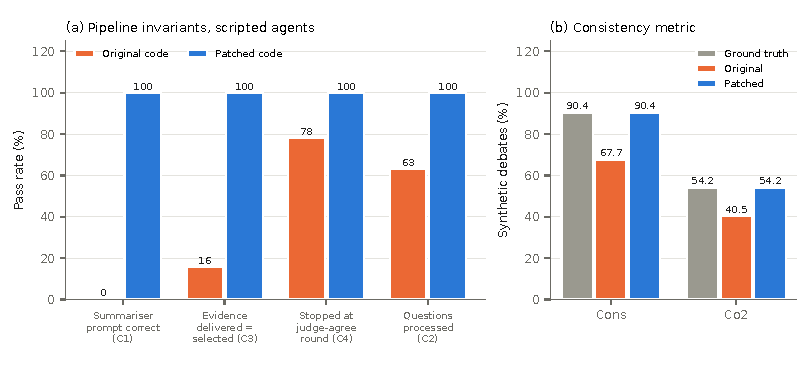
\includegraphics[width=\textwidth]{fig2_invariants_consistency}
\caption{(a) Invariant pass rates under scripted agents (TriviaQA; the scripted agents are index-based, so the rates are identical on all five datasets). (b) Consistency metrics against ground truth.}
\label{fig:invariants}
\end{figure}

\begin{table}[!htbp]
\centering
\small
\caption{Invariants, no injected failures (original = MADKE, patched = MADKE-X).}
\label{tab:invariants}
\resizebox{\textwidth}{!}{%
\begin{tabular}{lrrrrrrrr}
\toprule
 & \multicolumn{2}{c}{Processed} & \multicolumn{2}{c}{Summariser slot} & \multicolumn{2}{c}{Evidence delivered} & \multicolumn{2}{c}{Stop round} \\
\cmidrule(lr){2-3}\cmidrule(lr){4-5}\cmidrule(lr){6-7}\cmidrule(lr){8-9}
Dataset & Orig. & Patched & Orig. & Patched & Orig. & Patched & Orig. & Patched \\
\midrule
TriviaQA & 101 & 160 & 0\% & 100\% & 16\% & 100\% & 78\% & 100\% \\
NQ       & 101 & 160 & 0\% & 100\% & 16\% & 100\% & 78\% & 100\% \\
HotpotQA & 101 & 160 & 0\% & 100\% & 16\% & 100\% & 78\% & 100\% \\
2WikiMQA & 101 & 160 & 0\% & 100\% & 16\% & 100\% & 78\% & 100\% \\
FEVER    & 101 & 160 & 0\% & 100\% & 16\% & 100\% & 78\% & 100\% \\
\bottomrule
\end{tabular}%
}
\end{table}

\subsection{Evidence ordering}
Table~\ref{tab:ordering} and Figure~\ref{fig:ordering} show the share of questions with an answer-bearing passage among the first $k$; Table~\ref{tab:paired} gives the paired test. The ordering of MADKE (Wikipedia first) is below random on three of four sets, and RRF is above the random expectation on all four.

\begin{table}[!htbp]
\centering
\scriptsize
\caption{Consistency metrics against ground truth, with and without 3\% injected API failures.}
\label{tab:consistency}
\setlength{\tabcolsep}{3.5pt}
\resizebox{\textwidth}{!}{%
\begin{tabular}{llrrrrrrrrrr}
\toprule
 & & \multicolumn{4}{c}{Cons (\%)} & \multicolumn{4}{c}{Co2 (\%)} & \multicolumn{2}{c}{Failures} \\
\cmidrule(lr){3-6}\cmidrule(lr){7-10}\cmidrule(lr){11-12}
 & API & \multicolumn{2}{c}{Original} & \multicolumn{2}{c}{Patched} & \multicolumn{2}{c}{Original} & \multicolumn{2}{c}{Patched} & Scored & Flagged \\
\cmidrule(lr){3-4}\cmidrule(lr){5-6}\cmidrule(lr){7-8}\cmidrule(lr){9-10}
Dataset & fail & truth & metric & truth & metric & truth & metric & truth & metric & as text & (patched) \\
\midrule
TriviaQA & 0\% & 87.1 & 52.5 & 87.5 & 87.5 & 87.1 & 52.5 & 87.5 & 87.5 & 0 & 0 \\
TriviaQA & 3\% & 80.2 & 51.5 & 87.3 & 87.3 & 76.2 & 47.5 & 87.3 & 87.3 & 19 & 26 \\
NQ & 0\% & 87.1 & 52.5 & 87.5 & 87.5 & 87.1 & 52.5 & 87.5 & 87.5 & 0 & 0 \\
NQ & 3\% & 80.2 & 51.5 & 87.3 & 87.3 & 76.2 & 47.5 & 87.3 & 87.3 & 19 & 26 \\
HotpotQA & 0\% & 87.1 & 52.5 & 87.5 & 87.5 & 87.1 & 52.5 & 87.5 & 87.5 & 0 & 0 \\
HotpotQA & 3\% & 80.2 & 51.5 & 87.3 & 87.3 & 76.2 & 47.5 & 87.3 & 87.3 & 19 & 26 \\
2WikiMQA & 0\% & 87.1 & 52.5 & 87.5 & 87.5 & 87.1 & 52.5 & 87.5 & 87.5 & 0 & 0 \\
2WikiMQA & 3\% & 80.2 & 51.5 & 87.3 & 87.3 & 76.2 & 47.5 & 87.3 & 87.3 & 19 & 26 \\
FEVER & 0\% & 87.1 & 52.5 & 87.5 & 87.5 & 87.1 & 52.5 & 87.5 & 87.5 & 0 & 0 \\
FEVER & 3\% & 80.2 & 51.5 & 87.3 & 87.3 & 76.2 & 47.5 & 87.3 & 87.3 & 19 & 26 \\
\bottomrule
\end{tabular}%
}
\end{table}

\begin{figure}[!htbp]
\centering
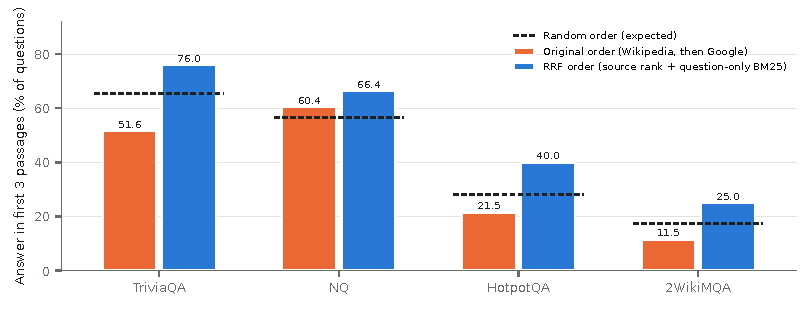
\includegraphics[width=\textwidth]{fig3_ordering}
\caption{Answer in the first three passages: MADKE order versus RRF order; the dashed line is the random-order expectation.}
\label{fig:ordering}
\end{figure}

\subsection{Cost: time, memory and tokens}
Table~\ref{tab:cost} and Figure~\ref{fig:cost} compare the two systems on all 500 questions of each dataset. The paper-sized pool reduces the evidence listing in every selection call by 44.8--45.3\% (mean 45.0\%; tokens estimated as characters/4, since no tokenizer was available); with at most six selection calls per question this is up to about 4,829 fewer input tokens per question on TriviaQA (4,841 on NQ), an upper bound because early stopping removes rounds. Ordering costs 0.68\,ms per question against 0.016\,ms for slicing, and peak memory is 6.9\,MB against 6.8\,MB. The parsers take 2.9 against 2.2 microseconds per call. These costs are negligible against the seconds a model call takes. We report no speed-up: in the zero-latency harness the per-question loop time (2.5\,ms for MADKE-X, 3.6\,ms with verification, 7.0\,ms for MADKE) is dominated by the harness matching questions in prompts, whose time grows with prompt length, and is therefore not a measure of system speed. The smaller pool is not free: it lowers the share of questions with any answer-bearing passage by 0.8 points (TriviaQA) to 3.4 points (NQ and HotpotQA) (Table~\ref{tab:poolcfg}).

\begin{table}[!htbp]
\centering
\small
\caption{Ordering on the shipped pools (percent of questions; MRR of the first answer-bearing passage).}
\label{tab:ordering}
\begin{tabular}{llrrrr}
\toprule
Dataset & Ordering & cov@1 & cov@3 & cov@5 & MRR \\
\midrule
\multirow{5}{*}{TriviaQA} & Original & 38.6 & 51.6 & 57.2 & 0.496 \\
 & Interleaved & 38.6 & 71.2 & 77.4 & 0.565 \\
 & BM25 & 53.6 & 75.0 & 79.0 & 0.646 \\
 & RRF & 55.2 & 76.0 & 79.2 & 0.657 \\
 & Random & 38.1 & 65.4 & 75.2 & 0.534 \\
\midrule
\multirow{5}{*}{NQ} & Original & 46.8 & 60.4 & 67.2 & 0.567 \\
 & Interleaved & 46.8 & 69.0 & 75.8 & 0.596 \\
 & BM25 & 35.4 & 62.8 & 73.0 & 0.513 \\
 & RRF & 44.2 & 66.4 & 75.0 & 0.571 \\
 & Random & 29.7 & 56.6 & 68.9 & 0.462 \\
\midrule
\multirow{5}{*}{HotpotQA} & Original & 15.9 & 21.5 & 24.9 & 0.225 \\
 & Interleaved & 15.9 & 33.5 & 39.4 & 0.269 \\
 & BM25 & 22.8 & 38.9 & 44.7 & 0.316 \\
 & RRF & 26.9 & 40.0 & 45.4 & 0.340 \\
 & Random & 12.9 & 28.2 & 36.7 & 0.228 \\
\midrule
\multirow{5}{*}{2WikiMQA} & Original & 6.4 & 11.5 & 15.0 & 0.126 \\
 & Interleaved & 6.4 & 21.6 & 28.6 & 0.165 \\
 & BM25 & 17.7 & 26.5 & 31.0 & 0.233 \\
 & RRF & 16.0 & 25.0 & 31.4 & 0.223 \\
 & Random & 7.0 & 17.4 & 25.1 & 0.148 \\
\bottomrule
\end{tabular}
\end{table}

\begin{table}[!htbp]
\centering
\small
\caption{Paired comparison, RRF versus MADKE order, cov@3.}
\label{tab:paired}
\setlength{\tabcolsep}{4pt}
\resizebox{\textwidth}{!}{%
\begin{tabular}{lrrrrcc}
\toprule
Dataset & $n$ & RRF only & Original only & Gain (pts) & 95\% bootstrap CI & Exact McNemar $p$ \\
\midrule
TriviaQA & 500 & 130 & 8 & $+24.4$ & [20.4, 28.4] & $1.6\times10^{-29}$ \\
NQ & 500 & 79 & 49 & $+6.0$ & [1.8, 10.6] & 0.010 \\
HotpotQA & 465 & 93 & 7 & $+18.5$ & [14.6, 22.4] & $2.7\times10^{-20}$ \\
2WikiMQA & 468 & 82 & 19 & $+13.5$ & [9.2, 17.7] & $1.7\times10^{-10}$ \\
\bottomrule
\end{tabular}%
}
\end{table}

\begin{table}[!htbp]
\centering
\small
\caption{Cost of MADKE (wiki 10 + Google 5, raw) and MADKE-X (paper pool, dedupe, RRF) on the shipped data.}
\label{tab:cost}
\setlength{\tabcolsep}{4pt}
\resizebox{\textwidth}{!}{%
\begin{tabular}{lrrrrrrr}
\toprule
 & \multicolumn{3}{c}{Evidence listing (est.\ tokens)} & \multicolumn{2}{c}{Pool build (ms/question)} & \multicolumn{2}{c}{Peak memory (MB)} \\
\cmidrule(lr){2-4}\cmidrule(lr){5-6}\cmidrule(lr){7-8}
Dataset & MADKE & MADKE-X & $-$\% & MADKE & MADKE-X & MADKE & MADKE-X \\
\midrule
TriviaQA & 1,778 & 973 & 45.3 & 0.014 & 0.646 & 7.0 & 6.5 \\
NQ & 1,801 & 994 & 44.8 & 0.017 & 0.598 & 6.7 & 6.2 \\
HotpotQA & 1,809 & 998 & 44.9 & 0.013 & 0.692 & 6.9 & 7.6 \\
2WikiMQA & 1,778 & 975 & 45.1 & 0.015 & 0.734 & 6.8 & 7.8 \\
FEVER & 1,793 & 987 & 45.0 & 0.020 & 0.709 & 6.8 & 6.3 \\
\bottomrule
\end{tabular}%
}
\end{table}

\begin{figure}[!htbp]
\centering
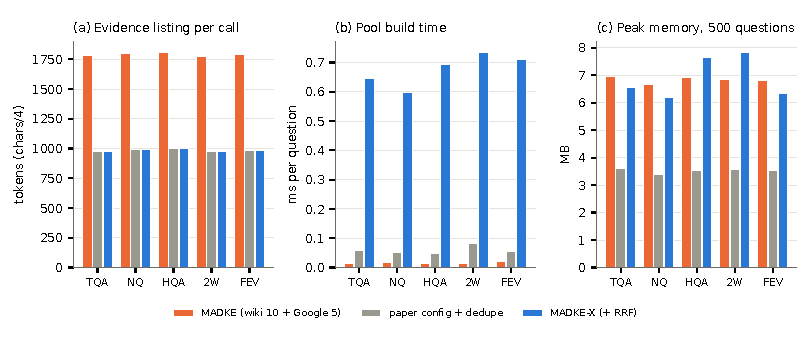
\includegraphics[width=\textwidth]{fig4_cost}
\caption{Evidence listing size, pool build time and peak memory over 500 questions per dataset.}
\label{fig:cost}
\end{figure}

\begin{table}[!htbp]
\centering
\small
\caption{Pool configurations (coverage = questions with an answer-bearing passage).}
\label{tab:poolcfg}
\setlength{\tabcolsep}{4pt}
\resizebox{\textwidth}{!}{%
\begin{tabular}{llrrrr}
\toprule
Dataset & Pool configuration & Passages & Words & Coverage (\%) & Dupes removed \\
\midrule
\multirow{3}{*}{TriviaQA} & code default (wiki 10 + Google 5) & 14.54 & 1,142 & 83.2 & 0 \\
 & paper (wiki 5 + Google 5) & 9.54 & 628 & 82.4 & 0 \\
 & patched (wiki 5 + Google 5, de-duplicated) & 9.52 & 626 & 82.4 & 10 \\
\midrule
\multirow{3}{*}{NQ} & code default (wiki 10 + Google 5) & 14.99 & 1,159 & 86.4 & 0 \\
 & paper (wiki 5 + Google 5) & 9.99 & 643 & 83.0 & 0 \\
 & patched (wiki 5 + Google 5, de-duplicated) & 9.98 & 641 & 83.0 & 7 \\
\midrule
\multirow{3}{*}{HotpotQA} & code default (wiki 10 + Google 5) & 14.94 & 1,148 & 50.5 & 0 \\
 & paper (wiki 5 + Google 5) & 9.94 & 634 & 47.1 & 0 \\
 & patched (wiki 5 + Google 5, de-duplicated) & 9.93 & 633 & 47.1 & 7 \\
\midrule
\multirow{3}{*}{2WikiMQA} & code default (wiki 10 + Google 5) & 14.80 & 1,146 & 40.4 & 0 \\
 & paper (wiki 5 + Google 5) & 9.80 & 631 & 37.4 & 0 \\
 & patched (wiki 5 + Google 5, de-duplicated) & 9.78 & 629 & 37.4 & 9 \\
\bottomrule
\end{tabular}%
}
\end{table}

\subsection{Trace and verification (structure only)}
Over 800 scripted debates every trace matches the evidence actually delivered (320/320 selections per dataset), every citation resolves to the pool and to a selected passage, and adding citations never changes the final answer. Table~\ref{tab:verification} and Figure~\ref{fig:verification} show the verification step on scripted agents whose summariser first cites an arbitrary selected passage: verification is triggered only for unsupported answers, is adopted only when the retry is supported, and increases the number of supported answers (for example 29 to 44 of 160 on NQ). Because the scripts are not models, these counts illustrate that the mechanism works, not how often a real model would be helped.

\begin{table}[!htbp]
\centering
\small
\caption{Verification on scripted agents (160 questions per dataset).}
\label{tab:verification}
\setlength{\tabcolsep}{4pt}
\resizebox{\textwidth}{!}{%
\begin{tabular}{lrrrrrrr}
\toprule
 & \multicolumn{3}{c}{Citations only (of 160)} & \multicolumn{4}{c}{Citations + verification} \\
\cmidrule(lr){2-4}\cmidrule(lr){5-8}
Dataset & supported & not found & no citation & supported & retries & adopted & answers changed \\
\midrule
TriviaQA & 10 & 98 & 52 & 13 & 150 & 3 & 0 \\
NQ & 29 & 79 & 52 & 44 & 131 & 15 & 0 \\
HotpotQA & 13 & 95 & 52 & 31 & 147 & 18 & 0 \\
2WikiMQA & 3 & 105 & 52 & 11 & 157 & 8 & 0 \\
FEVER & 0 & 108 & 52 & 1 & 160 & 1 & 0 \\
\bottomrule
\end{tabular}%
}
\end{table}

\begin{figure}[!htbp]
\centering
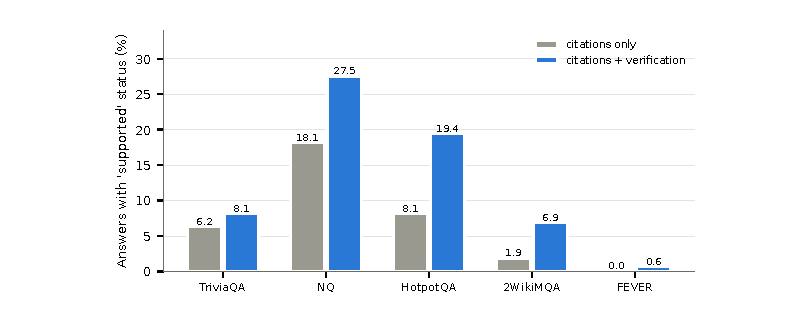
\includegraphics[width=\textwidth]{fig5_verification}
\caption{Supported answers with and without verification (scripted agents).}
\label{fig:verification}
\end{figure}
